\documentclass{article}

% PREAMBLE: This is where we load packages and set up the document's global properties.
\usepackage[letterpaper, margin=1in, textwidth=6.5in]{geometry} % For setting page margins and dimensions.
\usepackage{graphicx}       % To include images.
\usepackage{amsmath}        % For advanced math environments and symbols.
\usepackage{amssymb}        % For additional math symbols.
\usepackage{amsfonts}       % For math fonts.
\usepackage{enumitem}       % To customize lists (like itemize and enumerate).
\usepackage{pdfpages}       % To include external PDF pages.

% This command removes the page number from the first page (the title page).
\thispagestyle{empty}

% DOCUMENT TITLE
\title{Study Guide for the Chapters 5, 8, and 9 Quiz}

% We are not including an author or date for this study guide.
\author{}
\date{}

\begin{document}

\maketitle % This command generates the title based on the \title command above.

\subsection*{Quiz Details and Scope}
\begin{itemize}[itemsep=5pt]
    \item \textbf{Relevant Chapters:} This study guide covers the specified topics from Chapters 5, 8, and 9.
    \item \textbf{Quiz Format:} The quiz is closed-note.
    \item \textbf{Allowed Materials:} You are allowed a clean, unmarked copy of the provided periodic table. It is included at the end of this document for your convenience.
\end{itemize}

\subsection*{Key Topics for the Quiz}
This guide is focused exclusively on the following topics as outlined in \texttt{Exam 2 study topics.txt}.
\begin{itemize}[itemsep=5pt]
    \item \textbf{Chapter 5:} Ionic vs. Molecular Compounds, Lattice Energy, Predicting Formulas, Nomenclature (Ionic, Molecular, Acids, Hydrates), Polyatomic Ions, Empirical vs. Molecular Formulas, Molar Mass, Mass Percent, and various conversions (grams, moles, atoms).
    \item \textbf{Chapter 8:} Balancing Equations, Reaction Types, Combustion Analysis, Stoichiometry, Limiting \& Excess Reactants, and Theoretical \& Percent Yield.
    \item \textbf{Chapter 9:} Molarity Calculations, Dilutions, Solution Stoichiometry (Titrations), and pH/[H\(_3\)O\(^+\)] Calculations.
\end{itemize}

\bigskip
%========================================================================================
% STUDY PLAN SECTION
%========================================================================================
\subsection*{Phase 1: Foundation \& Memorization}
Your first step is to master the fundamental rules and definitions. Without this foundation, the practice problems will be very difficult.
\begin{itemize}[itemsep=5pt]
    \item Review the rules for classifying and naming compounds. The summary flowchart on \textbf{slide 42 of "Chapter 5 Ionic and Covalent Compounds.pdf"} is an excellent starting point.
    \item \textbf{Memorize the Polyatomic Ions}. This is critical. Use the chart on \textbf{slide 36 of "Chapter 5 Ionic and Covalent Compounds.pdf"}. Focus on the ions that are not crossed out. Making flashcards is highly effective.
    \item \textbf{Memorize Molecular Prefixes}. Review the Greek prefixes (mono-, di-, tri-, etc.) on \textbf{slide 23 of "Chapter 5 Ionic and Covalent Compounds.pdf"}.
    \item \textbf{Memorize Main-Group Element Charges}. The periodic table on \textbf{slide 9 of "Chapter 5 Ionic and Covalent Compounds.pdf"} shows the common charges for main-group elements. Knowing these is essential for writing correct ionic formulas.
    \item Understand the definitions of molarity, dilution, and pH. Refer to \textbf{slides 3, 7, and 17 of "Chapter 9 Chemical reactions in aqueous solutions.pdf"}.
    \item Review the definitions of limiting reactant, theoretical yield, and percent yield from \textbf{"Chapter 8 Chemical Reactions.pdf" (slides 32, 34, 42)}.
\end{itemize}

\bigskip
\subsection*{Phase 2: Practice \& Application}
Now, apply your knowledge by working through practice problems. Focus on understanding the \textit{process}, not just the answer.
\begin{itemize}[itemsep=5pt]
    \item Work through the practice problems in the provided worksheets. Key documents for this quiz are:
    \begin{itemize}
        \item \texttt{Ionic Nomenclature.pdf}
        \item \texttt{Covalent, hydrate, and acid nomenclature.pdf}
        \item \texttt{Empirical and Molecular Formulae.pdf}
        \item \texttt{Limiting Reagent Worksheet.pdf}
        \item \texttt{Molarity, dilutions, and solution stoichiometry.pdf}
    \end{itemize}
    \item Pay special attention to problems that combine multiple concepts, such as limiting reactant problems that also ask for percent yield.
    \item Review the detailed explanations of key problems in the next section of this guide to ensure you understand the step-by-step process.
\end{itemize}

\bigskip
\subsection*{Phase 3: Final Mastery}
In this final phase, simulate the test environment and solidify your knowledge.
\begin{itemize}[itemsep=5pt]
    \item Re-work the practice problems from Phase 2 without looking at the answer key. Try to explain each step to yourself as you go.
    \item Use the provided list of end-of-chapter problems from \texttt{Exam 2 study topics.txt} for additional practice on targeted areas where you feel less confident.
    \item \textbf{Final Step:} Print a clean, unmarked copy of \texttt{Periodic Table for testing.pdf}. This is the only tool you will have during the quiz.
\end{itemize}

\bigskip
%========================================================================================
% PROBLEM EXPLANATIONS SECTION
%========================================================================================
\subsection*{Explanations of Practice Problems}

\subsubsection*{Ionic Nomenclature with a Transition Metal}
\textbf{Problem:} Provide a complete name for CrS\(_3\). (From \texttt{Ionic Nomenclature.pdf}, Page 1, \#1d)

\textbf{Explanation:}
\begin{enumerate}[itemsep=5pt]
    \item \textbf{Identify the components:} The compound is made of Chromium (Cr), a transition metal, and Sulfur (S), a nonmetal. This means it's an ionic compound.
    \item \textbf{Determine the anion's charge:} Sulfur is in Group 16. Based on the periodic table trends, it forms an anion with a \textbf{-2 charge} (S\(^{2-}\)).
    \item \textbf{Determine the cation's charge:} The overall charge of an ionic compound must be neutral (zero). We have three sulfide ions, so the total negative charge is \(3 \times (-2) = -6\). To balance this, the single chromium ion must have a \textbf{+6 charge} (Cr\(^{6+}\)).
    \item \textbf{Name the compound:}
    \begin{itemize}
        \item Name the cation first: Chromium.
        \item Because Chromium is a transition metal that can have multiple charges, we must specify its charge with a Roman numeral in parentheses: \textbf{Chromium (VI)}.
        \item Name the anion by taking its root ("sulf-") and adding the "-ide" suffix: \textbf{sulfide}.
    \end{itemize}
    \item \textbf{Final Answer:} The complete name is \textbf{Chromium (VI) sulfide}.
\end{enumerate}

\bigskip
\subsubsection*{Limiting Reactants, Theoretical Yield, Excess, and Percent Yield}
\textbf{Problem:} From \texttt{Limiting Reagent Worksheet.pdf} (Page 1, \#1): Given the reaction CuCl\(_2\) + 2 NaNO\(_3\) \(\rightarrow\) Cu(NO\(_3\))\(_2\) + 2 NaCl. If 15.0 g of CuCl\(_2\) react with 20.0 g of NaNO\(_3\), answer the following.

\textbf{Part (b) - Find the limiting reagent and theoretical yield of Cu(NO\(_3\))\(_2\):}
\begin{enumerate}[itemsep=5pt]
    \item \textbf{Goal:} Determine which reactant runs out first by calculating how much product each reactant can create. The one that produces less is the limiting reagent.
    \item \textbf{Step 1: Molar Masses.} CuCl\(_2\) = 134.45 g/mol; NaNO\(_3\) = 84.99 g/mol; Cu(NO\(_3\))\(_2\) = 187.56 g/mol.
    \item \textbf{Step 2: Calculate product from CuCl\(_2\).}
    \[ 15.0 \text{ g CuCl}_2 \times \frac{1 \text{ mol CuCl}_2}{134.45 \text{ g CuCl}_2} \times \frac{1 \text{ mol Cu(NO}_3)_2}{1 \text{ mol CuCl}_2} \times \frac{187.56 \text{ g Cu(NO}_3)_2}{1 \text{ mol Cu(NO}_3)_2} \approx 20.9 \text{ g Cu(NO}_3)_2 \]
    \item \textbf{Step 3: Calculate product from NaNO\(_3\).}
    \[ 20.0 \text{ g NaNO}_3 \times \frac{1 \text{ mol NaNO}_3}{84.99 \text{ g NaNO}_3} \times \frac{1 \text{ mol Cu(NO}_3)_2}{2 \text{ mol NaNO}_3} \times \frac{187.56 \text{ g Cu(NO}_3)_2}{1 \text{ mol Cu(NO}_3)_2} \approx 22.1 \text{ g Cu(NO}_3)_2 \]
    \item \textbf{Step 4: Conclusion.} Since 15.0 g of CuCl\(_2\) produces less product (20.9 g) than 20.0 g of NaNO\(_3\) does, \textbf{CuCl\(_2\) is the limiting reagent}. The maximum amount of product that can be made is \textbf{20.9 g Cu(NO\(_3\))\(_2\)}, which is the \textbf{theoretical yield}.
\end{enumerate}

\textbf{Part (c) - Find the amount of excess reagent (NaNO\(_3\)) left over:}
\begin{enumerate}[itemsep=5pt]
    \item \textbf{Goal:} Use the limiting reagent to determine how much of the other reactant was actually used, then subtract that from the starting amount.
    \item \textbf{Step 1: Calculate mass of NaNO\(_3\) used.} Start with the initial mass of the limiting reagent (CuCl\(_2\)) and convert it to the mass of the excess reagent (NaNO\(_3\)) that reacted with it.
    \[ 15.0 \text{ g CuCl}_2 \times \frac{1 \text{ mol CuCl}_2}{134.45 \text{ g CuCl}_2} \times \frac{2 \text{ mol NaNO}_3}{1 \text{ mol CuCl}_2} \times \frac{84.99 \text{ g NaNO}_3}{1 \text{ mol NaNO}_3} \approx 19.0 \text{ g NaNO}_3 \text{ used} \]
    \item \textbf{Step 2: Calculate mass remaining.} Subtract the used mass from the starting mass.
    \[ \text{Mass left} = \text{Initial Mass} - \text{Used Mass} = 20.0 \text{ g} - 19.0 \text{ g} = \textbf{1.0 g NaNO\(_3\)} \]
\end{enumerate}

\textbf{Part (d) - Calculate the percent yield if 11.3 g of Cu(NO\(_3\))\(_2\) are formed:}
\begin{enumerate}[itemsep=5pt]
    \item \textbf{Goal:} Use the percent yield formula. The "actual yield" is what was experimentally formed (11.3 g). The "theoretical yield" is what we calculated in part (b) (20.9 g).
    \[ \text{Percent Yield} = \frac{\text{Actual Yield}}{\text{Theoretical Yield}} \times 100\% = \frac{11.3 \text{ g}}{20.9 \text{ g}} \times 100\% \approx \textbf{54.0\%} \]
\end{enumerate}

\bigskip
\subsubsection*{Solution Stoichiometry (Titration)}
\textbf{Problem:} What is the volume (in mL) of 1.2 M HCl needed to dissolve 5.8 g Al(OH)\(_3\)? The balanced reaction is: Al(OH)\(_3\)(s) + 3 HCl(aq) \(\rightarrow\) AlCl\(_3\)(aq) + 3 H\(_2\)O(l). (From \texttt{Molarity, dilutions, and solution stoichiometry.pdf}, Page 2, \#6)

\textbf{Explanation:} This is a stoichiometry problem that starts with a solid and asks for the volume of a solution.
\begin{enumerate}[itemsep=5pt]
    \item \textbf{Goal:} Convert the mass of Al(OH)\(_3\) to the volume of HCl solution needed. The path is: g Al(OH)\(_3\) \(\rightarrow\) mol Al(OH)\(_3\) \(\rightarrow\) mol HCl \(\rightarrow\) L HCl \(\rightarrow\) mL HCl.
    \item \textbf{Step 1: Molar Mass of Al(OH)\(_3\).} 26.98 + 3(16.00 + 1.008) = 78.00 g/mol.
    \item \textbf{Step 2: Convert mass of Al(OH)\(_3\) to moles.}
    \[ 5.8 \text{ g Al(OH)}_3 \times \frac{1 \text{ mol Al(OH)}_3}{78.00 \text{ g Al(OH)}_3} \approx 0.07436 \text{ mol Al(OH)}_3 \]
    \item \textbf{Step 3: Use stoichiometric ratio to find moles of HCl.} From the balanced equation, the ratio is 3 mol HCl to 1 mol Al(OH)\(_3\).
    \[ 0.07436 \text{ mol Al(OH)}_3 \times \frac{3 \text{ mol HCl}}{1 \text{ mol Al(OH)}_3} \approx 0.2231 \text{ mol HCl} \]
    \item \textbf{Step 4: Use molarity to find volume of HCl.} Molarity (M) = mol/L, so Volume (L) = mol / M.
    \[ V = \frac{0.2231 \text{ mol HCl}}{1.2 \text{ mol/L}} \approx 0.1859 \text{ L HCl} \]
    \item \textbf{Step 5: Convert Liters to Milliliters.}
    \[ 0.1859 \text{ L} \times \frac{1000 \text{ mL}}{1 \text{ L}} \approx \textbf{190 mL} \text{ (rounded to two significant figures)} \]
\end{enumerate}

\bigskip
\subsubsection*{pH and [H\(_3\)O\(^+\)] Calculations}
\textbf{Problem:} Calculate the pH for a solution with [H\(_3\)O\(^+\)] = 8.82 x 10\(^{-4}\) M. Is it acidic or basic? (From \texttt{Chapter 9 Chemical reactions in aqueous solutions.pdf}, Slide 19)

\textbf{Explanation:}
\begin{enumerate}[itemsep=5pt]
    \item \textbf{Formula:} The formula relating pH and hydronium ion concentration is \textbf{pH = -log[H\(_3\)O\(^+\)]}.
    \item \textbf{Calculation:} Substitute the given concentration into the formula.
    \[ \text{pH} = -\log(8.82 \times 10^{-4}) \approx 3.054 \]
    \item \textbf{Significant Figures:} The concentration (8.82 x 10\(^{-4}\)) has three significant figures. For pH calculations, the number of significant figures in the concentration corresponds to the number of \textbf{decimal places} in the pH value. Therefore, the answer should have 3 decimal places.
    \item \textbf{Acidity:} A pH less than 7.00 is acidic. A pH greater than 7.00 is basic. Since 3.054 is less than 7, the solution is \textbf{acidic}.
    \item \textbf{Final Answer:} The pH is \textbf{3.054}, and the solution is \textbf{acidic}.
\end{enumerate}


% This command creates a new page so the PDF can be included cleanly.
\newpage

% This command includes the specified PDF file, showing all its pages.
% Replace 'Periodic Table for testing.pdf' if your filename is different.
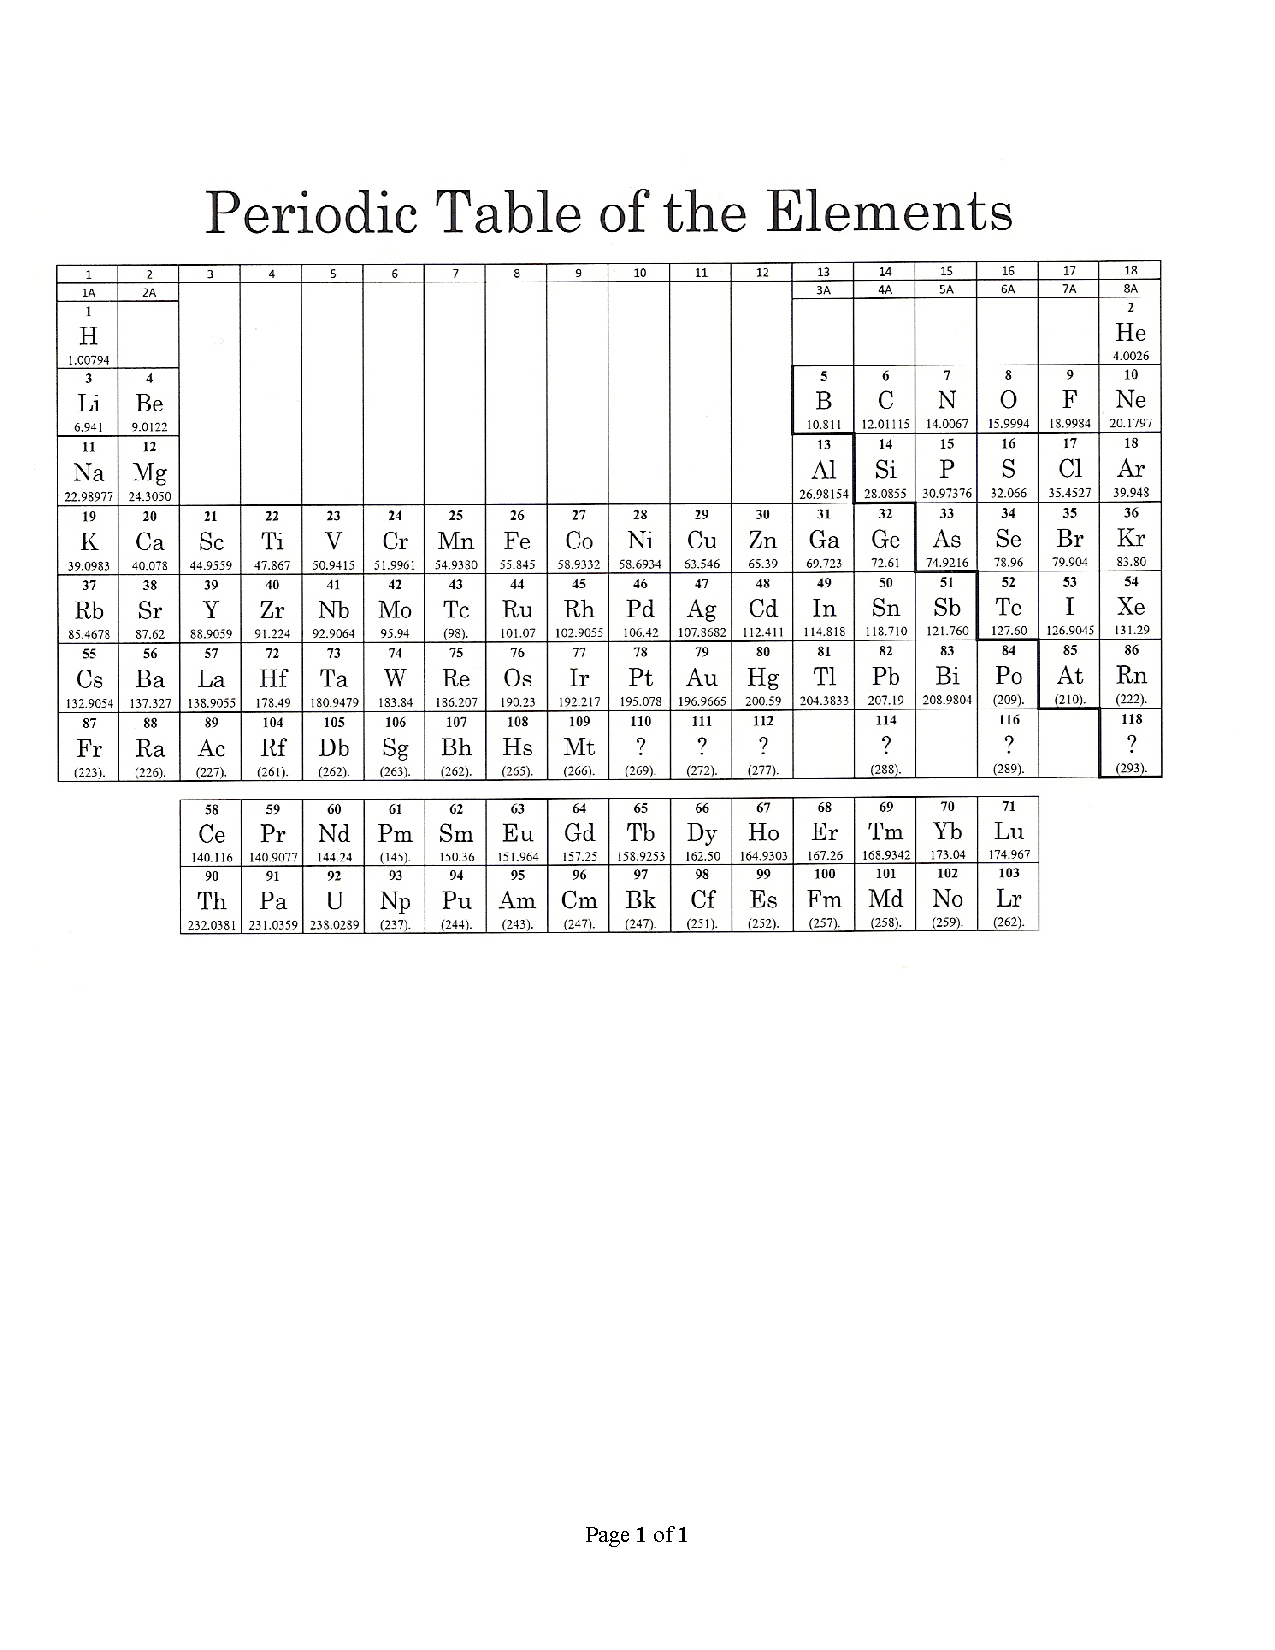
\includepdf[pages={-}]{Periodic Table for testing.pdf}

\end{document}